\begin{exercises}
	% Topics:
	% Spans
	% Representing lines/planes/volumes as spans
	% translated spans
	% linear independence
	
	\begin{problist}
		\prob Let $A=\Set*{\mat{1\\2\\0},\mat{0\\1\\0},\mat{1\\1\\0}}$.
		\begin{enumerate}
			\item Is $A$
			linearly independent or dependent?
			
			\item Describe the span of $A$.
			
			\item Can $A$ be extended (i.e., can vectors be added to $A$) so that
			$A$ spans all of $\R^3$?
		\end{enumerate}
		\begin{solution}
			\begin{enumerate}
				\item Linearly dependent
				\item $\Span(A)$ is the plane $\Set*{\mat{x \\y \\0} \in\R^3: x,y\in\R}$
				\item Yes. If B = $A\cup\Set*{\mat{0\\0\\1}}$, then $\Span(B)=\R^3$
			\end{enumerate}
		\end{solution}
		
		\prob For each set below, determine whether it spans a point,
		line, plane, volume, or other. \label{PROBSET3-SETS}
		\begin{enumerate}
			\item $\Set*{\mat{1\\1}}$
			
			\item $\Set*{\mat{1\\3},\mat{2\\6}}$
			
			\item $\Set*{\mat{2\\4},\mat{4\\2}}$
			
			\item $\Set*{\mat{1\\2},\mat{-1\\-2}}$
			
			\item $\Set*{\mat{1\\2},\mat{-1\\2}}$
			
			\item $\Set*{}$
			
			\item $\Set*{\mat{1\\2},\mat{2\\3},\mat{3\\4}}$
			
			\item $\Set*{\mat{5\\4\\-3},\mat{1\\1\\0},\mat{2\\2\\2}}$
			
			\item $\Set*{\mat{1\\-2\\0},\mat{4\\-5\\1}}$
			
			\item $\Set*{\mat{1\\-2\\0},\mat{4\\-5\\1},\mat{5\\-7\\1}}$
		\end{enumerate}
		\begin{solution}
			\begin{enumerate}
				\item Line
				\item Line
				\item Plane
				\item Line
				\item Plane
				\item Point
				\item Plane
				\item Volume
				\item Plane
				\item Plane
			\end{enumerate}
		\end{solution}
		
		\prob
		\begin{enumerate}
			\item For each set in question \ref{PROBSET3-SETS}, determine whether it is
			linearly independent or dependent.
			
			\item Is the set $\Set*{\mat{1\\2\\3},\mat{5\\6\\7},
				\mat{9\\10\\11}, \mat{13\\14\\15}}$ linearly
			independent or dependent?
			
			\item Can you find a set of $n+1$ vectors in $\R^{n}$ that is linearly independent? Explain.
		\end{enumerate}
		\begin{solution}
			\begin{enumerate}
				\item
				\begin{enumerate*}
					\item Linearly Independent
					\item Linearly Dependent
					\item Linearly Independent
					\item Lineraly Dependent
					\item Linearly Independent
					\item Linearly Independent
					\item Linearly Dependent
					\item Linearly Independent
					\item Linearly Independent
					\item Linearly Dependent
				\end{enumerate*}
				\item Linearly Dependent
				\item No. The solutions to the vector equation
				$\alpha_{1}\vec x_{1}+\alpha_{2}\vec x_{2}+\ldots+\alpha_{n+1}\vec x_{n+1}=0$
				for $\alpha_{1},\alpha_{2},\ldots,\alpha_{n+1} \in \R$
				are the solutions to a system of $n$ equations
				in $n+1$ variables. This system is consistent
				since
				$\alpha_{1}=\alpha_{2}=\ldots=\alpha_{n+1}=0$
				is a solution. The row reduced echelon form
				of the corresponding augmented matrix has at
				least one free variable column since there are more
				columns than rows. Hence there are
				infinitely many solutions, and in particular
				there exists a non-trivial solution to the
				above vector equation.
			\end{enumerate}
		\end{solution}
		
		\prob
		\begin{enumerate}
			\item If possible, express the following lines in $\R^{2}$
			as spans. Otherwise, justify why the line cannot
			be expressed as a span. \label{PROBSET3-R2-spans}
			\begin{enumerate}
				\item $x=0$
				
				\item $2x+3y=0$
				
				\item $5x-4y=0$
				
				\item $-x-y=-1$ \label{PROBSET3-R2-iv}
				
				\item $9x-15y=8$ \label{PROBSET3-R2-v}
			\end{enumerate}
			
			\item For each line in question \ref{PROBSET3-R2-spans} that cannot
			be expressed as a span, express it as a translated
			span.
			
			\item Each equation below specifies a line or a plane in $\R^3$. If possible,
			express the specified line or plane as a span. Otherwise,
			justify
			why it cannot be expressed as a span. \label{PROBSET3-R3-spans}
			\begin{enumerate}
				\item $2x-y+z=4$ \label{PROBSET3-R3-i}
				
				\item $x+6y-z=0$
				
				\item $x+3z=0$
				
				\item $y=1$ \label{PROBSET-R3-iv}
				
				\item $x=0$ and $z=0$
				
				\item $2x-y=2$ and $z=-1$ \label{PROBSET3-R3-vi}
			\end{enumerate}
			
			\item For lines or planes in question \ref{PROBSET3-R3-spans} that cannot
			be expressed as spans, express as a translated
			span.
		\end{enumerate}
		\begin{solution}
			\begin{enumerate}
				\item
				\begin{enumerate}
					\item $\Span\Set*{\mat{0\\-1}}$
					\item $\Span\Set*{\mat{3\\-2}}$
					\item $\Span\Set*{\mat{4\\5}}$
					\item Not possible since \[\mat{0\\0}\notin \Set*{\mat{x\\y}\in \R^2: -x-y=-1}.\]
					\item Not possible since $\mat{0\\0}$ is not on the line.
				\end{enumerate}
				\item
				\ref{PROBSET3-R2-iv} $\Span\Set*{\mat{1\\-1}} + \Set*{\mat{1\\0}}$;
				\ref{PROBSET3-R2-v} $\Span\Set*{\mat{5\\3}} + \Set*{\mat{8/9\\0}}$
				\item 
				\begin{enumerate}
					\item Impossible since $\vec 0$ is not in the plane.
					\item $\Span\Set*{\mat{6\\-1\\0}, \mat{1\\0\\1}}$
					\item $\Span\Set*{\mat{3\\0\\-1}, \mat{0\\1\\0}}$
					\item Impossible since $\vec 0$ is not in the plane.
					\item $\Span\Set*{\mat{0\\1\\0}}$
					\item Impossible since $\vec 0$ is not in the plane.
				\end{enumerate}
				\item 
					\ref{PROBSET3-R3-i} $\Span\Set*{\mat{1\\2\\0}, \mat{0\\1\\1}} + \Set*{\mat{2\\0\\0}}$;
					\ref{PROBSET-R3-iv} $\Span\Set*{\mat{1\\0\\0}, \mat{0\\0\\1}} + \Set*{\mat{0\\1\\0}}$;
					\ref{PROBSET3-R3-vi} $\Span\Set*{\mat{1\\2\\0}} + \Set*{\mat{1\\0\\-1}}$
			\end{enumerate}
		\end{solution}
		
		\prob Determine if the following planes, expressed in vector form, are the same plane.
		\begin{enumerate}
			\item $\vec x = t\mat{1\\2}+ s\mat{2\\7}$ and $\vec x =
			t\mat{3\\5}+ s\mat{8\\4}$.
			
			\item $\vec x = t\mat{2\\2\\3}+ s\mat{1\\0\\5}$ and $\vec
			x = t\mat{1\\0\\5}+ s\mat{4\\2\\13}$.
			
			\item $\vec x = t\mat{1\\2\\1}+ s\mat{2\\2\\1}$ and $\vec
			x = t\mat{0\\1\\0}+ s\mat{1\\2\\1}$.
		\end{enumerate}
		\begin{solution}
			\begin{enumerate}
				\item Same plane ($\R^2$).
				\item Same plane ($2\mat{1\\0\\5} + \mat{2\\2\\3} = \mat{4\\2\\13}$).
				\item Different plane ($\mat{2\\2\\1}$ is not in the second plane).
			\end{enumerate}
		\end{solution}
		
		\prob Show that the set $\Set*{\mat{2\\0\\7},\mat{1\\1\\1},\mat{6\\4\\11}}$
		is linearly dependent in two ways. First, using the geometric definition of linear dependence
		and then using the algebraic definition.
		\begin{solution}
			The set is linearly dependent since: $\mat{6\\4\\11}=
			\mat{2\\0\\7}+ 4\mat{1\\1\\1}$ (geometric) or
			$\mat{2\\0\\7}+ 4\mat{1\\1\\1}+ (-1)\mat{6\\4\\11}=\vec 0$.
		\end{solution}
		
		\prob Choose vectors $\vec p$, $\vec d_{1}$, $\vec d_{2}$,
		$\vec d_{3}$ in $\R^{4}$ such that the vector equation
		$\vec x = t_{1}\vec d_{1} + t_{2}\vec d_{2} + t_{3}\vec d_{3}+\vec p$ specifies:
		\begin{enumerate}
			\item A hyperplane passing through the origin.
			
			\item A plane not passing through the origin.
			
			\item A line passing through the origin.
			
			\item The point $(2,2,2,3)$.
		\end{enumerate}
		\begin{solution}
			$\vec {x} = t_{1}\vec {d}_{1}+t_{2}\vec {d}_{2}+t_{3}\vec {d}_{3}+t_{4}\vec {d}_{4}+\vec {p}$
			\begin{enumerate}
				\item $\vec{d}_{1}= \mat{1\\0\\0\\0}$,
				$\vec{d}_{2}= \mat{0\\1\\0\\0}$, $\vec{d}_{3}=\mat{0\\0\\1\\0}$,
				$\vec{p}= \mat{0\\0\\0\\0}$
				\item $\vec{d}_{1}= \mat{1\\0\\0\\0}$, and
				$\vec{d}_{2}= \mat{0\\1\\0\\0}$, $\vec{d}_{3}=\mat{1\\1\\0\\0}$,
				$\vec{p}= \mat{0\\0\\1\\0}$
				\item $\vec{d}_{1}= \mat{1\\0\\0\\0}$,
				$\vec{d}_{2}= \mat{2\\0\\0\\0}$, $\vec{d}_{3}=
				\mat{-1\\0\\0\\0}$, $\vec{p}= \mat{0\\0\\0\\0}$
				\item $\vec {d}_{1} = \vec {d}_{2} = \vec {d}_{3} = \vec {0}$, 
				$\vec {p} = \mat{2\\2\\2\\3}$
			\end{enumerate}
		\end{solution}

		\prob Classify the sets $A=\Set{}$ and $B=\Set{\vec 0}$ as linearly independent or dependent.
		\begin{solution}
			The set $A$ is linearly independent. Since $A$ contains no vectors, there is no way to
			write $\vec 0$ as a non-trivial linear combination of vectors in $A$. However, $B$ is linearly
			dependent, since $\vec 0=7\vec 0$ is a non-trivial linear combination of vectors in $B$ that give
			the zero vector.
		\end{solution}
		
		\prob Let $S=\Set*{\mat{1\\3},\mat{0\\-1}}$ and let $T=\Set*{\mat{-1\\-1},\mat{0\\2},\mat{0\\0}}$. Draw
		the sets $S$, $T$, and $T+S$.
		\begin{solution}			
			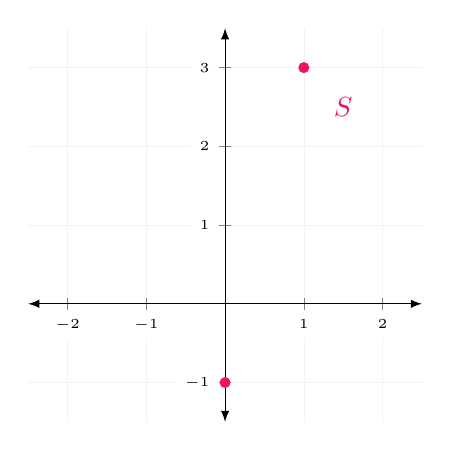
\begin{tikzpicture}[baseline = (current bounding box.north)]
				\begin{axis}[
					anchor=origin,
					disabledatascaling,
					xmin=-2,xmax=2,
					ymin=-1,ymax=3,
					xtick={-2,...,2},
					ytick={-1,...,3},
					x=1cm,y=1cm,
					grid=both,
					grid style={line width=.1pt, draw=gray!10},
					%major grid style={line width=.2pt,draw=gray!50},
					axis lines=middle,
					minor tick num=0,
					enlargelimits={abs=0.5},
					axis line style={latex-latex},
					ticklabel style={font=\tiny,fill=white},
					xlabel style={at={(ticklabel* cs:1)},anchor=north west},
					ylabel style={at={(ticklabel* cs:1)},anchor=south west}
				]
					\fill [WildStrawberry] (1,3) circle (2pt);
					\fill [WildStrawberry] (0,-1) circle (2pt);
				\end{axis}
				\node [WildStrawberry] at (1.5,2.5) {$S$};
			\end{tikzpicture}
			
			\begin{tikzpicture}[baseline = (current bounding box.north)]
				\begin{axis}[
					anchor=origin,
					disabledatascaling,
					xmin=-2,xmax=2,
					ymin=-1,ymax=3,
					xtick={-2,...,2},
					ytick={-1,...,3},
					x=1cm,y=1cm,
					grid=both,
					grid style={line width=.1pt, draw=gray!10},
					%major grid style={line width=.2pt,draw=gray!50},
					axis lines=middle,
					minor tick num=0,
					enlargelimits={abs=0.5},
					axis line style={latex-latex},
					ticklabel style={font=\tiny,fill=white},
					xlabel style={at={(ticklabel* cs:1)},anchor=north west},
					ylabel style={at={(ticklabel* cs:1)},anchor=south west}
				]
					\fill [mygreen] (0,0) circle (2pt);
					\fill [mygreen] (-1,-1) circle (2pt);
					\fill [mygreen] (0,2) circle (2pt);
				\end{axis}
				\node [mygreen] at (1.5,2.5) {$T$};
			\end{tikzpicture}
			
			\begin{tikzpicture}[baseline = (current bounding box.north)]
				\begin{axis}[
					anchor=origin,
					disabledatascaling,
					xmin=-4,xmax=4,
					ymin=-2,ymax=6,
					xtick={-4,-2,0,2,4},
					ytick={-2,0,2,4,6},
					x=0.5cm,y=0.5cm,
					grid=both,
					grid style={line width=.1pt, draw=gray!10},
					%major grid style={line width=.2pt,draw=gray!50},
					axis lines=middle,
					minor tick num=0,
					enlargelimits={abs=1},
					axis line style={latex-latex},
					ticklabel style={font=\tiny,fill=white},
					xlabel style={at={(ticklabel* cs:1)},anchor=north west},
					ylabel style={at={(ticklabel* cs:1)},anchor=south west}
				]
					\fill [myorange] (0,2) circle (2pt);
					\fill [myorange] (-1,-2) circle (2pt);
					\fill [myorange] (1,5) circle (2pt);
					\fill [myorange] (0,1) circle (2pt);
					\fill [myorange] (1,3) circle (2pt);
					\fill [myorange] (0,-1) circle (2pt);
				\end{axis}
				\node [myorange] at (1.5,2.5) {$T+S$};
			\end{tikzpicture}
		\end{solution}
		
		\prob Let $S=\Set*{\mat{1\\1},\mat{0\\-1}, \mat{0\\0}}$. 
		\begin{enumerate}
			\item 
			Draw $S$, $S+S$, and $(S+S)+S$.
			\item Is $(S+S)+S=S+(S+S)$? Does the expression $S+S+S$ make sense?
			\item Draw $S+S+S+S+\cdots$.
		\end{enumerate}
		\begin{solution}
			\begin{enumerate}
				\item 
				The set $S$:
				
				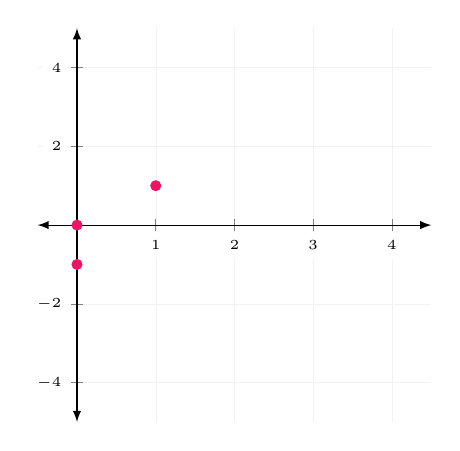
\begin{tikzpicture}[baseline = (current bounding box.north)]
					\begin{axis}[
						anchor=origin,
						disabledatascaling,
						xmin=0,xmax=4,
						ymin=-4,ymax=4,
						xtick={0,...,4},
						ytick={-4,-2,0,2,4},
						x=1cm,y=0.5cm,
						grid=both,
						grid style={line width=.1pt, draw=gray!10},
						%major grid style={line width=.2pt,draw=gray!50},
						axis lines=middle,
						minor tick num=0,
						enlarge x limits={abs=0.5},
						enlarge y limits={abs=1.0},
						axis line style={latex-latex},
						ticklabel style={font=\tiny,fill=white},
						xlabel style={at={(ticklabel* cs:1)},anchor=north west},
						ylabel style={at={(ticklabel* cs:1)},anchor=south west}
					]
						\fill [WildStrawberry] (1,1) circle (2pt);
						\fill [WildStrawberry] (0,-1) circle (2pt);
						\fill [WildStrawberry] (0,0) circle (2pt);
					\end{axis}
				\end{tikzpicture}
				
				The set $S+S$:
				
				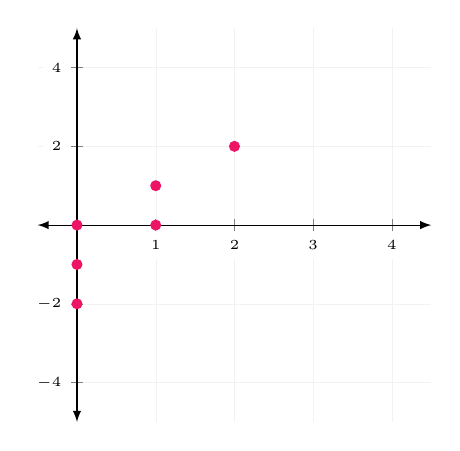
\begin{tikzpicture}[baseline = (current bounding box.north)]
					\begin{axis}[
						anchor=origin,
						disabledatascaling,
						xmin=0,xmax=4,
						ymin=-4,ymax=4,
						xtick={0,...,4},
						ytick={-4,-2,0,2,4},
						x=1cm,y=0.5cm,
						grid=both,
						grid style={line width=.1pt, draw=gray!10},
						%major grid style={line width=.2pt,draw=gray!50},
						axis lines=middle,
						minor tick num=0,
						enlarge x limits={abs=0.5},
						enlarge y limits={abs=1.0},
						axis line style={latex-latex},
						ticklabel style={font=\tiny,fill=white},
						xlabel style={at={(ticklabel* cs:1)},anchor=north west},
						ylabel style={at={(ticklabel* cs:1)},anchor=south west}
					]
						\fill [WildStrawberry] (2,2) circle (2pt);
						\fill [WildStrawberry] (1,0) circle (2pt);
						\fill [WildStrawberry] (0,-2) circle (2pt);
						\fill [WildStrawberry] (1,1) circle (2pt);
						\fill [WildStrawberry] (0,-1) circle (2pt);
						\fill [WildStrawberry] (0,0) circle (2pt);
					\end{axis}
				\end{tikzpicture}
				
				The set $(S+S)+S$:
				
				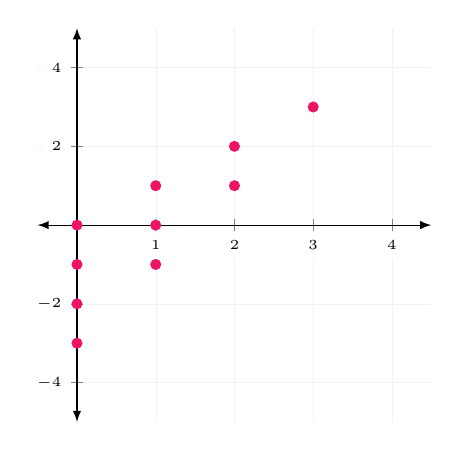
\begin{tikzpicture}[baseline = (current bounding box.north)]
					\begin{axis}[
						anchor=origin,
						disabledatascaling,
						xmin=0,xmax=4,
						ymin=-4,ymax=4,
						xtick={0,...,4},
						ytick={-4,-2,0,2,4},
						x=1cm,y=0.5cm,
						grid=both,
						grid style={line width=.1pt, draw=gray!10},
						%major grid style={line width=.2pt,draw=gray!50},
						axis lines=middle,
						minor tick num=0,
						enlarge x limits={abs=0.5},
						enlarge y limits={abs=1.0},
						axis line style={latex-latex},
						ticklabel style={font=\tiny,fill=white},
						xlabel style={at={(ticklabel* cs:1)},anchor=north west},
						ylabel style={at={(ticklabel* cs:1)},anchor=south west}
					]
						\fill [WildStrawberry] (0,-3) circle (2pt);
						\fill [WildStrawberry] (0,-2) circle (2pt);
						\fill [WildStrawberry] (0,-1) circle (2pt);
						\fill [WildStrawberry] (0,0) circle (2pt);
						\fill [WildStrawberry] (1,-1) circle (2pt);
						\fill [WildStrawberry] (1,0) circle (2pt);
						\fill [WildStrawberry] (1,1) circle (2pt);
						\fill [WildStrawberry] (2,1) circle (2pt);
						\fill [WildStrawberry] (2,2) circle (2pt);
						\fill [WildStrawberry] (3,3) circle (2pt);
					\end{axis}
				\end{tikzpicture}
				\item The set $(S+S)+S$ and $S+(S+S)$ are equal since vector addition is associative. This means that $S+S+S$ is well-defined and we can drop the parentheses, so the expression $S+S+S$ makes sense.
				\item 
				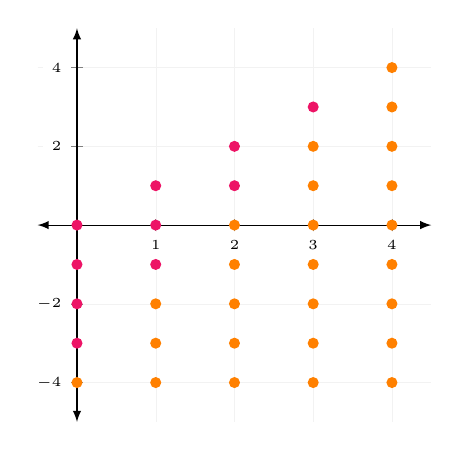
\begin{tikzpicture}[baseline = (current bounding box.north)]
					\begin{axis}[
						anchor=origin,
						disabledatascaling,
						xmin=0,xmax=4,
						ymin=-4,ymax=4,
						xtick={0,...,4},
						ytick={-4,-2,0,2,4},
						x=1cm,y=0.5cm,
						grid=both,
						grid style={line width=.1pt, draw=gray!10},
						%major grid style={line width=.2pt,draw=gray!50},
						axis lines=middle,
						minor tick num=0,
						enlarge x limits={abs=0.5},
						enlarge y limits={abs=1.0},
						axis line style={latex-latex},
						ticklabel style={font=\tiny,fill=white},
						xlabel style={at={(ticklabel* cs:1)},anchor=north west},
						ylabel style={at={(ticklabel* cs:1)},anchor=south west}
					]
						\fill [WildStrawberry] (0,-3) circle (2pt);
						\fill [WildStrawberry] (0,-2) circle (2pt);
						\fill [WildStrawberry] (0,-1) circle (2pt);
						\fill [WildStrawberry] (0,0) circle (2pt);
						\fill [WildStrawberry] (1,-1) circle (2pt);
						\fill [WildStrawberry] (1,0) circle (2pt);
						\fill [WildStrawberry] (1,1) circle (2pt);
						\fill [WildStrawberry] (2,1) circle (2pt);
						\fill [WildStrawberry] (2,2) circle (2pt);
						\fill [WildStrawberry] (3,3) circle (2pt);
					\end{axis}
					\foreach \x [evaluate=\x as \ymax using 2*\x] in {0,...,4} {
						\foreach \y in {0,...,\ymax} {
							\fill [orange] (\x,-2+\y/2) circle (2pt);
						}
					}
				\end{tikzpicture}
				
				Notice that we obtain the orange points when we add an additional $S$ to the set sum. Since we are considering the infinite sum $S+S+S+S+\cdots$, the process continues infinitely.
			\end{enumerate}
		\end{solution}
		
		\prob Let $D\subseteq\R^2$ be the unit disk centered at the origin and let $L\subseteq \R^2$ be
		the line segment from $(0,0)$ to $(0,2)$.
		\begin{enumerate}
			\item How many points are in $D$, $L$, and $D+L$?
			\item Draw $D+L$.
			\item Find the area of $D+L$.
			\item Suppose $S\subseteq\R^2$ makes a smiley face when drawn and the ``thickness'' of
			each line composing this smiley face is $0.01$ units. Can you find a set $A$ so
			that the set $S+A$ represents a smiley face where the lines have a thickness of $0.05$?
			If so, give an example of such an $A$. Otherwise, explain why it is impossible.
		\end{enumerate}
		\begin{solution}
			\begin{enumerate}
				\item There are infinitely many points in each of D, L, and $D+L$.
				\item 
				\begin{tikzpicture}[baseline = (current bounding box.north)]
					\begin{axis}[
						anchor=origin,
						disabledatascaling,
						xmin=-2,xmax=2,
						ymin=-1,ymax=3,
						xtick={-2,...,2},
						ytick={-1,...,3},
						x=1cm,y=1cm,
						grid=both,
						grid style={line width=.1pt, draw=gray!10},
						%major grid style={line width=.2pt,draw=gray!50},
						axis lines=middle,
						minor tick num=0,
						enlargelimits={abs=0.5},
						axis line style={latex-latex},
						ticklabel style={font=\tiny,fill=white},
						xlabel style={at={(ticklabel* cs:1)},anchor=north west},
						ylabel style={at={(ticklabel* cs:1)},anchor=south west}
					]
						\fill [mygreen, opacity=.3] (0,0) -- (-1,0) arc (180:360:1.0cm) -- cycle;
						\fill [mygreen, opacity=.3] (0,2) -- (1,2) arc (0:180:1.0cm) -- cycle;
						\fill [mygreen, opacity=.3] (1,0) -- (-1,0) -- (-1,2) -- (1,2) -- cycle;
					\end{axis}
					\node [mygreen] at (1.5,1.5) {$D+L$};
				\end{tikzpicture}
				\item $D+L$ can be decomposed into $2$ unit radius half-circles and a square with side length
				$2$. The area of $D+L$ is then $\pi+4$.
				\item We can take A to be a circle of radius $0.02$ units.
			\end{enumerate}
		\end{solution}
		
		\prob Let $\vec v_{1}, \vec v_{2}, \vec v_{3}$ be vectors. For each of the following statements,
		justify whether the statement is true or false.
		\begin{enumerate}
			\item If $\vec v_{1}$ can be written as a linear combination
			of $\vec v_{2}$ and $\vec v_{3}$, then $\Set{\vec
				v_1,\vec v_2,\vec v_3}$ is linearly dependent.
			
			\item If $\Set{\vec v_1,\vec v_2,\vec v_3}$ is linearly dependent,
			then $\vec v_{1}$ can be written as a linear combination
			of $\vec v_{2}$ and $\vec v_{3}$.
			
			\item If $\vec v_{1}=k\vec v_{2}$ for some real number $k$,
			then $\Set{\vec v_1,\vec v_2}$ is linearly dependent.
			
			\item If $\vec v_{1}$ is not a scalar multiple of $\vec
			v_{2}$, then $\Set{\vec v_1,\vec v_2,\vec v_3}$ is
			linearly independent.
			
			\item All spans contain $\vec 0$.
		\end{enumerate}
		\begin{solution}
			\begin{enumerate}
				\item True by the geometric definition of linear dependence.
				\item False. $\Set*{\mat{1\\0},\mat{0\\0},\mat{0\\1}}$ is linearly
				dependent, but $\mat{1\\0}$ is not a linear combination of $\mat{0\\0}$ and $\mat{0\\1}$.
				\item True. $\vec{v}_{1}$ is a linear combination of $\vec{v}_{2}$ and so 
				$\Set*{\vec {v}_{1},\vec{v}_{2}}$ is linearly dependent by the definition
				of linear dependence.
				\item False. $\Set*{\mat{1\\0},\mat{0\\0},\mat{0\\1}}$ is linearly dependent, 
				but $\mat{1\\0}$ is not a scalar multiple of $\mat{0\\1}$.
				\item True. The linear combination of any finite set with all coefficients zero is $\vec {0}$.
			\end{enumerate}
		\end{solution}
	\end{problist}
\end{exercises}
